\chapter{Data Structure}

    In programming, we encounter various data structures beyond what is available in languages like Python. In Python, we often use lists to perform a variety of operations such as \texttt{pop}, \texttt{add}, \texttt{remove}, and \texttt{concatenate}, without explicit concerns about list size. Additionally, Python allows flexible data typing (e.g., adding an integer to a float), making it a convenient but less controlled environment. 
    
    \section{Data Types}
    A \textbf{data type} specifies the nature of values and defines the operations allowed on those values. For instance, in Python, stacks, queues, deques, and linked lists are often managed under the umbrella of lists, which provides flexibility but less control.
    
    \section{List}
    A \textbf{list} is a sequential collection of values, where each element has a specific position (or index).
    Indexes range from 0 to n-1( there n is the length of the list) or from 1 to n. Lists in Python are heterogeneous, meaning they can store values of different types, whereas strings are homogeneous since their elements are characters.
    
    Python supports several operations on lists, each of which is an example of an Abstract Data Type (ADT):
    \begin{itemize}
        \item \texttt{list.append(x)}: Add an item to the end of the list.
        \item \texttt{list.extend(L)}: Extend the list by appending all items in the given list \(L\).
        \item \texttt{list.insert(i, x)}: Insert item \(x\) at position \(i\).The first argument is the index of the element before which to insert, so a.insert(0,x) inserts at the front of the list.
        \item \texttt{list.remove(x)}:Remove the first item from the list whose value is x. It is an error if there is no such item.
        \item \texttt{list.pop(i)}: Remove and return the item at position \(i\), if no index is specified, a.pop() removes and returns the last item in the list.
        \item \texttt{list.index(x)}: Return the index of the first item  whose value is \(x\).
        \item \texttt{list.count(x)}: Count occurrences of \(x\) in the list.
    \end{itemize}
    
    \section{Stack}
    A \textbf{stack} is a collection of objects following the Last-In-First-Out (LIFO) principle, where elements are added to the top and removed from the top. The height (length) of the stack refers to the number of elements, while the top represents the most recently added element.
    
    Stack ADT(Abstract Data Type):
    \begin{itemize}
        \item \texttt{S.push(e)}: Add element \(e\) to the top.
        \item \texttt{S.pop()}: Remove and return the top element.
        \item \texttt{S.top()}: Return the top element without removing it.
        \item \texttt{S.is\_empty()}: Check if the stack is empty.
        \item \texttt{len(S)}: Return the length of the stack.
    \end{itemize}
    
    \section{Queue}
    A \textbf{queue} is a collection of objects following the First-In-First-Out (FIFO) principle, where elements are added at the back and removed from the front.
    
    Queue ADT:
    \begin{itemize}
        \item \texttt{Q.enqueue(e)}: Add element \(e\) to the back of the queue.
        \item \texttt{Q.dequeue()}: Remove and return the front element.
        \item \texttt{Q.first()}: Return the front element without removing it.
        \item \texttt{Q.is\_empty()}: Check if the queue is empty.
        \item \texttt{len(Q)}: Return the length of the queue.
    \end{itemize}
    
    \section{Deque}
    A \textbf{deque} (double-ended queue) it's a queue where you can get the first() or the last() element and allows elements to be added or removed from both ends. Unlike lists, deques restrict access to middle elements.
    
    Deque ADT:
    \begin{itemize}
        \item \texttt{Q.add\_first(e)}: Add element \(e\) to the front.
        \item \texttt{Q.add\_last(e)}: Add element \(e\) to the back.
        \item \texttt{Q.delete\_first()}: Remove and return the front element.
        \item \texttt{Q.delete\_last()}: Remove and return the back element.
        \item \texttt{Q.first()}, \texttt{Q.last()}, \texttt{Q.is\_empty()}, \texttt{len(Q)}: Same as queue operations.
    \end{itemize}
    
    In Python, deques can be implemented using the \texttt{collections} module. For example, \texttt{append()} adds to the back, and \texttt{popleft()} removes from the front.Given a deque D in Python, you can get an element at index i as D[i]. Indexed access is \(O(1)\) at both ends but degrades to \(O(n)\) for elements in the middle.
    
    \section{Linked List}
    A \textbf{linked list} is a data structure where elements are stored in nodes linked together in a sequence by pointers. Unlike arrays, where the order is maintained by indexes, linked lists maintain order through pointers.
    
    \subsection{Singly Linked List}
    In a singly linked list, each node has a value and a pointer to the next node. The first node is the head, and the last node is the tail. Maintaining a pointer to the head is essential for accessing the list. Traversing a list means moving from the head to the tail. A Linked List must maintain a pointer to the head, otherwise there is no way to locate that node. Sometimes also a pointed to the tail is stored (to avoid traversal). List “nodes” are “objects”.

    

    \begin{figure}[H]
        \centering
        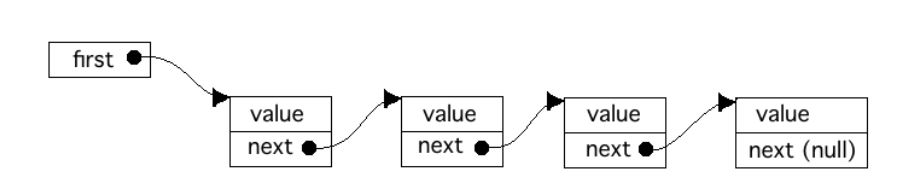
\includegraphics[width=0.5\linewidth]{immagini/singly linked list.JPG}
        \label{fig:enter-label}
    \end{figure}

    
    Adding a Node to a linked list
    \begin{enumerate}
        \item Create a new node, \texttt{newest = Node(e)}.
        \item Set \texttt{newest.next} to the current head:  \texttt{newest.next = L.head}
        \item Update \texttt{L.head} to point to \texttt{newest}.
        \item Increase the list size: \texttt{L.size=L.size+1}
    \end{enumerate}
    \begin{figure}[h!]
        \centering
        \begin{minipage}{0.45\textwidth}
          \centering
          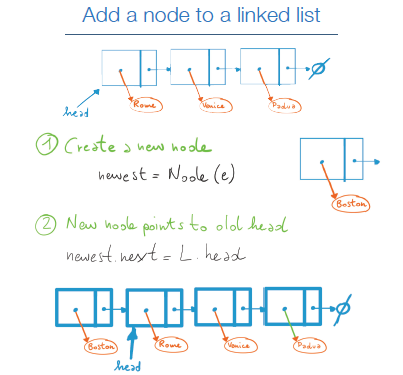
\includegraphics[width=\textwidth]{immagini/linkl1.png}
        \end{minipage}
        \hfill
        \begin{minipage}{0.45\textwidth}
          \centering
          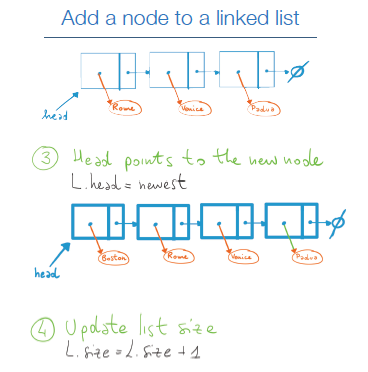
\includegraphics[width=\textwidth]{immagini/linkl2.png}
        \end{minipage}
        \label{fig:two_images}
    \end{figure}
    \newpage
    Removing a Node
    \begin{enumerate}
        \item Find the node with the value to remove (e.g., "Rome").
        \item Set \texttt{previous.next} to \texttt{current.next} and delete the current node.
    \end{enumerate}
    \begin{figure}[h!]
        \centering
        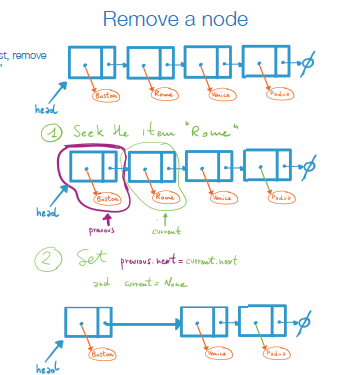
\includegraphics[width=0.5\linewidth]{immagini/linkl3.png}
    \end{figure}

    \subsection{Circularly Linked List}
    In a circularly linked list, the last node points back to the head, creating a circular structure. Be cautious with traversals as they loop infinitely.
    \begin{figure}[h]
        \centering
        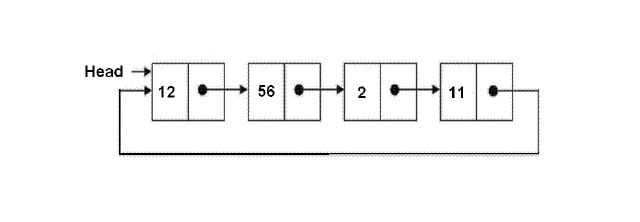
\includegraphics[width=0.8\linewidth]{immagini/circularly linked lists.JPG }
        \label{fig:enter-label}
    \end{figure}
    \newpage
    \subsection{Doubly Linked List}
    A doubly linked list has pointers in both directions, allowing traversal from both ends. It includes header and trailer nodes as sentinels, which simplify insertions.
    \begin{figure}[h!]
        \centering
        \begin{minipage}{0.7\textwidth}
          \centering
          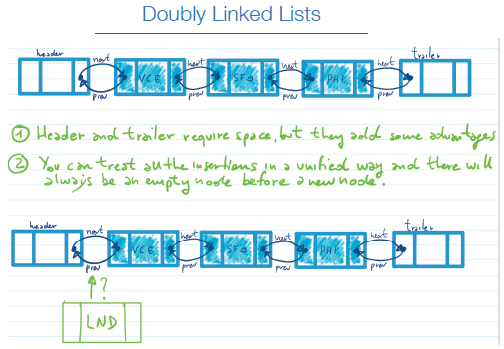
\includegraphics[width=\textwidth]{immagini/dlink1.png}
        \end{minipage}
        \hfill
        \begin{minipage}{0.7\textwidth}
          \centering
          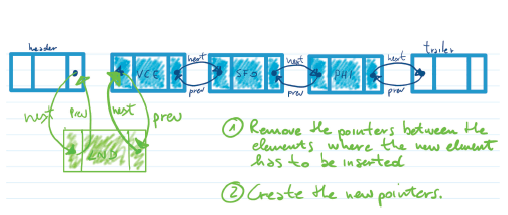
\includegraphics[width=\textwidth]{immagini/dlink2.png}
        \end{minipage}
        \label{fig:two_images}
    \end{figure}
    \subsection{Exercise: Find the Middle Node}
    Given a singly linked list of \(N\) nodes, find the middle node. If \(N\) is even, return the second middle element.
    
    \begin{itemize}
        \item Solution 1: Traverse the list and count nodes. Traverse again up to count/2 to find the middle node.
        \item Solution 2: Use two pointers, one moving twice as fast as the other. When the fast pointer reaches the end, the slow pointer is at the middle.
    \end{itemize}
    
    \subsection{Exercise: Check if a Linked List is a Palindrome}
    Given a singly linked list, check if it is a palindrome.
    
    \textbf{Solution}: Traverse the list, pushing each node onto a stack. Traverse again, popping elements from the stack and comparing each with the current node. If all match, return true.
    
    \subsection{Exercise: Reverse a Linked List}
    Given the head of a linked list, reverse the list.
    
    \textbf{Solution}:
    \begin{verbatim}
    current = head
    while current is not None:
        next = current.next
        current.next = prev
        prev = current
        current = next
    head = prev
    \end{verbatim}
    
    \subsection{Positional List}
    It is a data structure that allows us to perform arbitrary insertions and deletions or to refer to elements anywhere in a list. Numerical indexes are good, but they require to scan the entire list to find a specific element and to change dynamically when we update a list. An index does not always refer to the same element within a list. A positional list is an abstraction that provides the ability to identify the position of an element in a list.
    

    
    \section{Array vs. List-Based Data Structures}
    The complexity of those structure is different:
    \begin{itemize}
        \item Arrays: O(1)-time access to an element based on an index
        \item O(n) in a linked list to do the traversal
    \end{itemize}
    Also the storing consumption is different:
    \begin{itemize}
        \item Arrays: we may need to store 2n elements (dynamic resizing)
        \item Lists: we store n elements and n references (singly linked lists) and 2n references (doubly linked lists)
    \end{itemize}
    
    \begin{figure}[h]
        \centering
        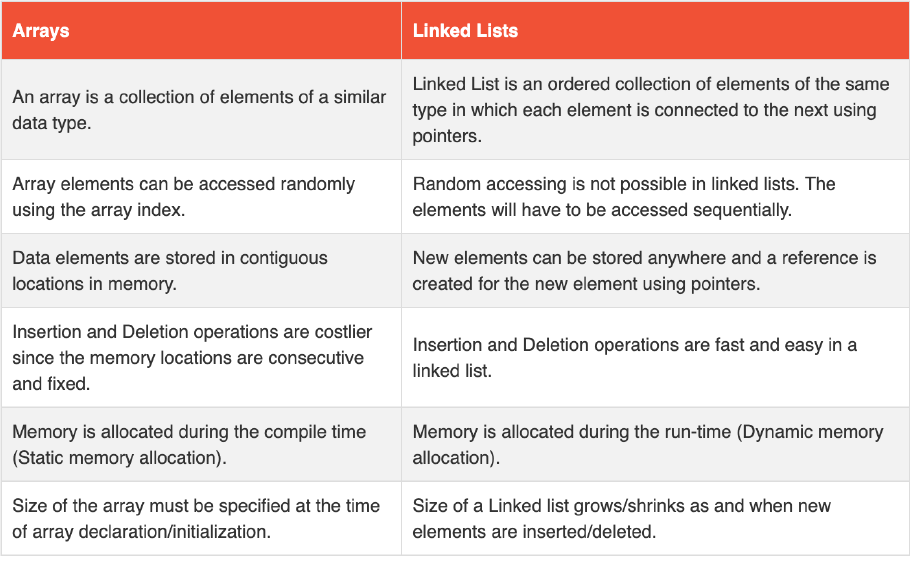
\includegraphics[width=0.9\linewidth]{immagini/06_data structure table .png}

    \end{figure}
        
    \section{Implementing Linked Lists with Arrays}

    \begin{enumerate}
        \item  Using Three Arrays: Implementation with three arrays:
                   \begin{itemize}
                       \item \texttt{next} keep the pointers to the next element.
                       \item \texttt{key} contains the actual elements.
                       \item \texttt{prev} stores the index of the previous element.
                   \end{itemize}
                Here, \texttt{L} maintains the index of the head.
        \item Using a Single Array: Represent objects in a contiguous sub-array \([j \dots k]\). Each attribute corresponds to an offset (e.g., key, next, prev), and the object's pointer is the starting index \(j\).
    \end{enumerate}
    \begin{figure}
        \centering
        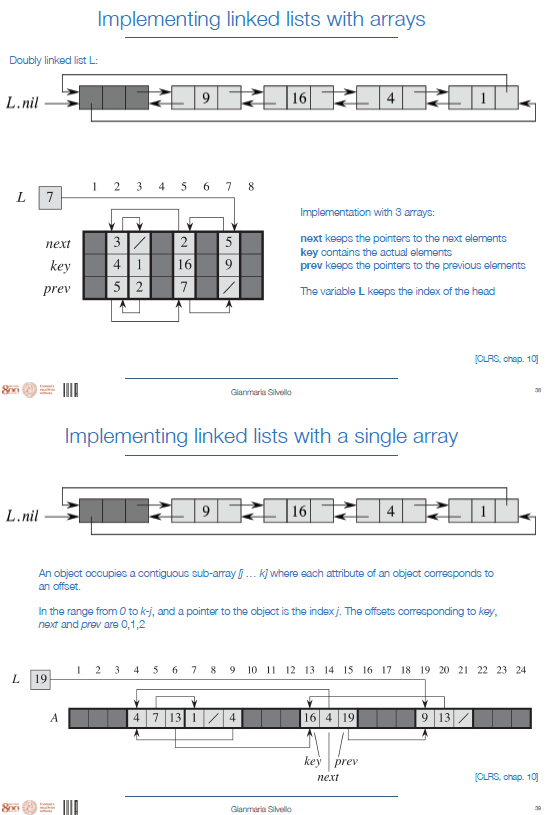
\includegraphics[width=1\linewidth]{immagini/listarray.png}
        \label{fig:enter-label}
    \end{figure}
    
    

    
    

